\section{Bibliometric Analysis Methodology}\label{sec:Bibliometric-Methodology}

To justify the focus on graph-based approaches in traffic forecasting, we conducted a systematic bibliometric analysis.

\subsection{Data Collection}

A broad search in Scopus using ``traffic forecast*'' retrieved approximately 60,000 documents. Filtering for peer-reviewed English articles in Engineering or Computer Science yielded 784 articles (2000--2025).

\subsection{Keyword Processing}

The 6,343 unique keywords were reduced to 217 (frequency $\geq$ 10). Semantic clustering using Sentence-BERT embeddings grouped these into 66 meaningful concept clusters. Similar terms (e.g., ``graph neural network'', ``GNN'') were unified.

\subsection{Key Findings}

\begin{figure}[ht]
\centering
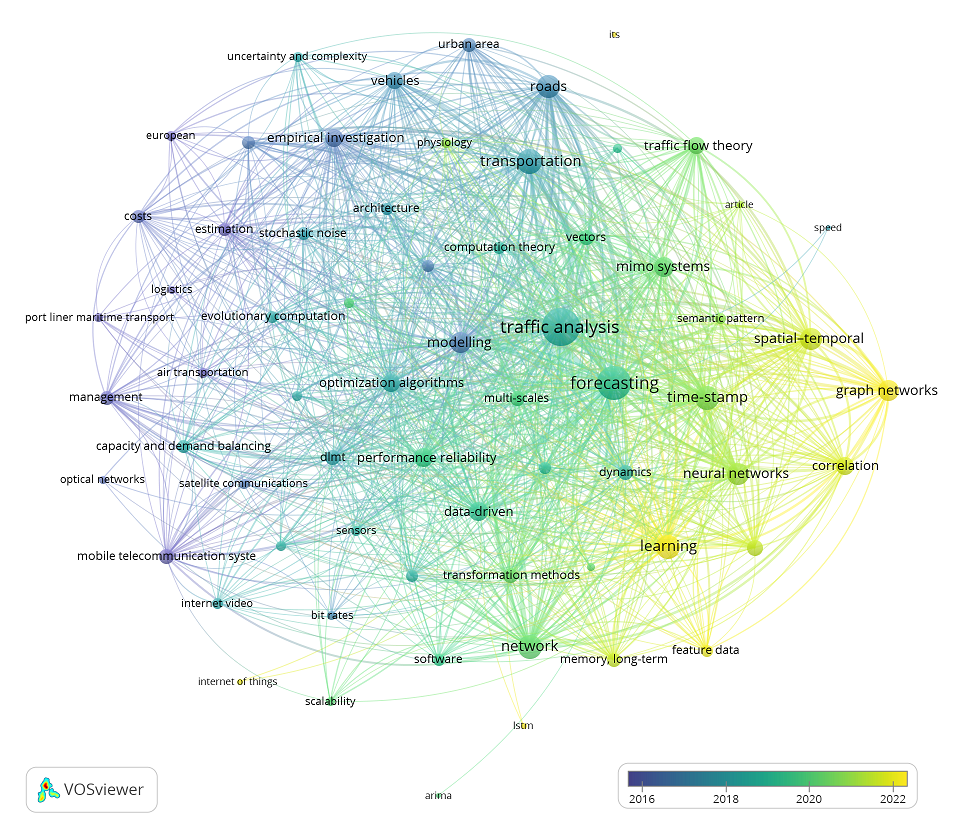
\includegraphics[width=0.9\linewidth]{scopus-clustered.png}
\caption{Clustered keyword co-occurrence network from 784 articles, colored by average publication year. Graph-based methods (right nodes) are the most recent focus.}
\label{fig:clustered_keywords}
\end{figure}

Figure~\ref{fig:clustered_keywords} reveals that graph-based methods have become the dominant recent methodological focus. However, nearly all rely on predefined graph structures---directly motivating our Graph Structure Learning approach.

\begin{figure}[ht]
\centering
\begin{subfigure}{0.32\textwidth}
    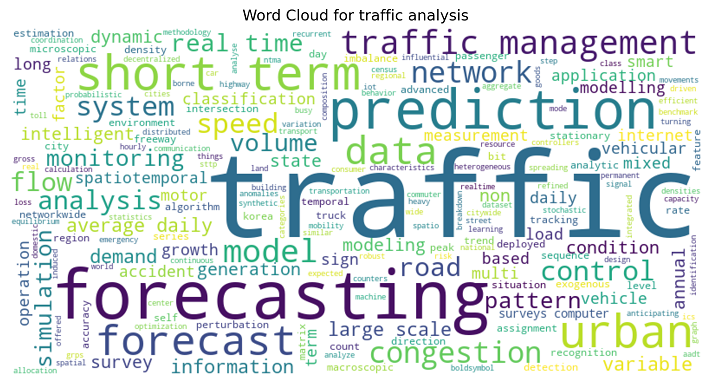
\includegraphics[width=\linewidth]{1-traffic analysis.png}
    \caption{Traffic Analysis}
\end{subfigure}
\hfill
\begin{subfigure}{0.32\textwidth}
    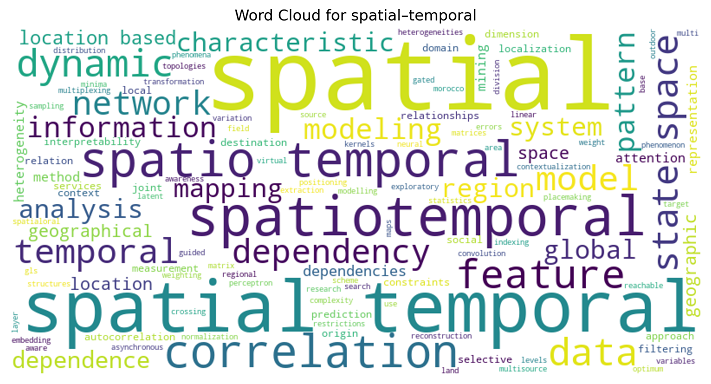
\includegraphics[width=\linewidth]{5-spatial–temporal.png}
    \caption{Spatio-Temporal}
\end{subfigure}
\hfill
\begin{subfigure}{0.32\textwidth}
    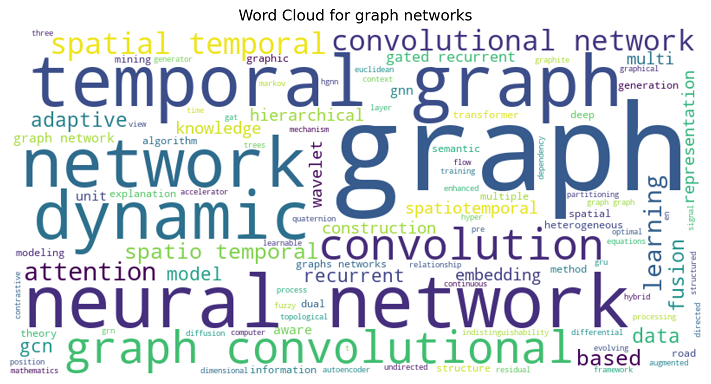
\includegraphics[width=\linewidth]{8-graph networks.png}
    \caption{Graph Networks}
\end{subfigure}
\caption{Word clouds from three key bibliometric clusters.}
\label{fig:word-clouds}
\end{figure}
